\documentclass[10pt]{article}
\usepackage[margin=1in]{geometry} 
\usepackage{amsmath,amsthm,amssymb,amsfonts}
\usepackage{graphicx}

\setlength{\parindent}{0pt}

\newcommand{\N}{\mathbb{N}}
\newcommand{\Z}{\mathbb{Z}}

\begin{document}

\title{COMP550 Natural Language Processing\\Assignment 1}
\author{Jonathan Guymont}
\maketitle

\section*{Question 1}
\textbf{Case 1}: "That's Wong on so many levels."\\

This is an \textit{orthographic} ambiguity. The sentence could be interpreted has \textit{there is a lot of peoples call Wong on all the floors} or has the common expression \textit{that is wrong on so many levels}. The word \textit{Wong} which could be mistaken for \textit{wrong} is the cause of ambiguity. Knowing that Names are starting by a capital letter could prevent a system from making a mistake. For instance, a spell checker would probably change wong for wrong otherwise. Having access to the context would also disambiguate the sentence. \\

\textbf{Source}: https://www.pinterest.ca/pin/360076932688489937/?lp=true\\

\textbf{Case 2}: "But I know what I am and I'm glad I'm a man, and so is Lola"\\

This is an \textit{Syntactic} ambiguity. The sentence could be interpreted has \textit{I am glad to be a man and Lola is glad to be a man} or has \textit{I am glad to be a man and Lola is glad I am a man}. The way the sentence is writen: \textit{I am glad I am [something], and so is [another person]} cause ambiguity. Without the context, knowing that Lola is more a woman name would disambiguate the passage.\\

\textbf{Source}: https://www.reddit.com/r/Music/comments/2izue5/serious\_is\_lola\_a\_transvestite/\\

\textbf{Case 3}: "GOP Lawmakers Grill IRS Chief Over Lost Emails"\\

This is a \textit{lexical} ambiguity. The sentence could be interpreted has \textit{GOP lawmakers are grilling the chief of IRS (has in burning over a fire) for losing emails} or has \textit{GOP lawmakers are giving a hard time (without any violence) to the chief of IRS}. The word \textit{Grill} is the cause of ambiguity. Knowing that US government employees do not get totured by the government disambiguate the passage.\\

\textbf{Source}: https://www.wsj.com/articles/gop-lawmakers-grill-irs-chief-over-loss-emails-1403278518?mg=id-wsj\\

\textbf{Case 4}: "you look like I need a drink"\\

This is a \textit{pragmatic} ambiguity. The sentence could be interpreted has \textit{I have a biological need to drink} or has \textit{I would like a drink}. The expression \textit{I need a drink} meaning \textit{I would like to have a drink} is the cause of ambiguity. Knowing the expression would disambiguate the passage.\\

\textbf{Source}: https://genius.com/Justin-moore-you-look-like-i-need-a-drink-lyrics\\

\textbf{Case 5}: "this is a big plane"\\

This is a \textit{phonological} ambiguity. The sentence could be interpreted has \textit{this is a big plain} or has \textit{this is a big plane}. The word \textit{plane} cause of ambiguity, because we use the same phonome to say \textit{plane} or \textit{plain}. Knowing the english level of the writer and the context would help determining the chance he or she meant \textit{plain}. \\

\textbf{Source}: http://livestly.com/new-worlds-largest-plane/\\

\section*{Question 2}
\begin{figure}[h!]
    \centering
    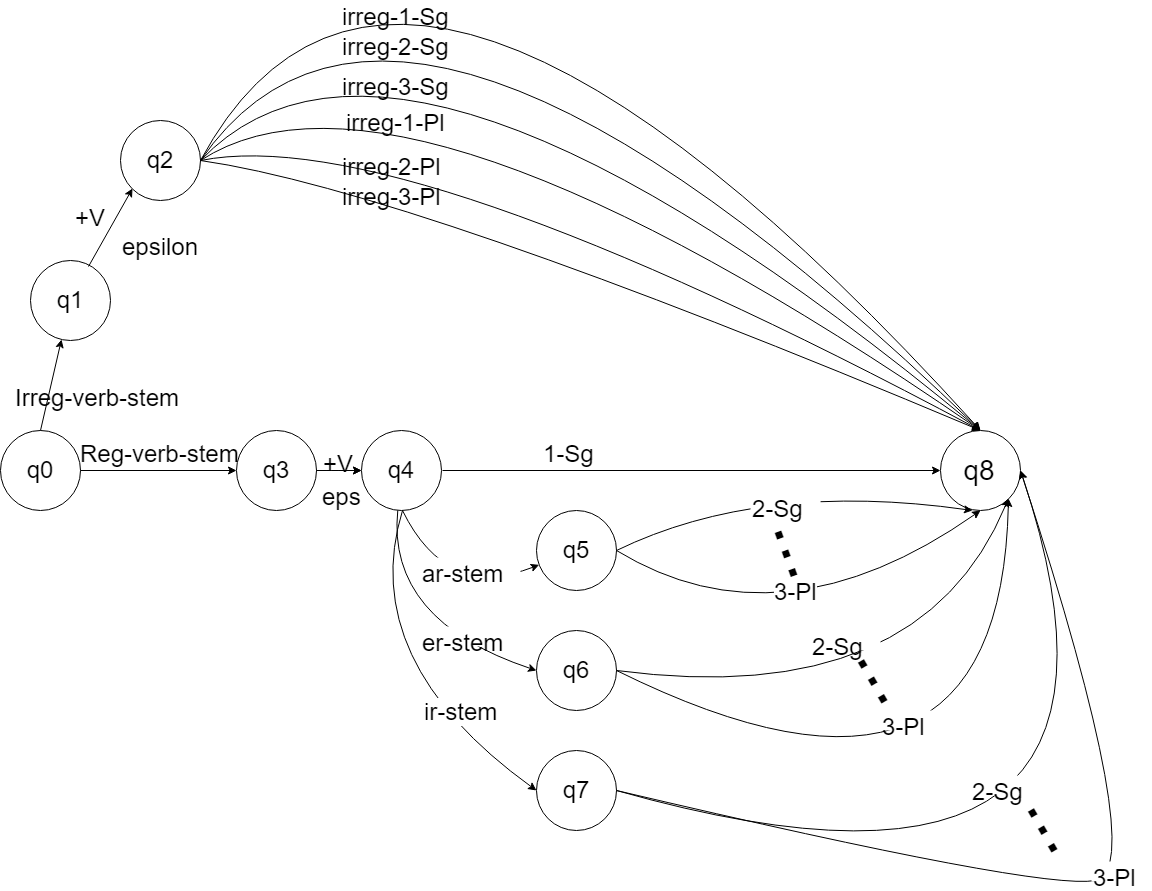
\includegraphics[scale=0.25]{schematic_transducer.png}
    \caption{Schematic Transducer}
    \label{fig:boat1}
\end{figure}

\begin{table}[h!]
\resizebox{\textwidth}{!}{
    \centering
    \begin{tabular}{ |c|c|c|c|c|c|c| } 
       \hline
        \textbf{infinitive}	&	\textbf{1-sg-reg}	&	\textbf{2-sg-reg}	&	\textbf{3-sg-reg}	&	\textbf{1-pl-reg}	&	\textbf{2-pl-reg}	&	\textbf{3-pl-reg}	\\ 
        \hline													
        andar	&	and a:o e:$\epsilon$	&	and a:a r:s	&	and a:a r:$\epsilon$	&	and a:a r:m $\epsilon$:o $\epsilon$:s	&	and a:á r:i $\epsilon$:s	&	and a:a r:n	\\ 
        \hline													
        contestar	&	contest a:o r:$\epsilon$ 	&	contest a:a r:s	&	contest a:a r:$\epsilon$	&	contest a:a r:m $\epsilon$:o $\epsilon$:s	&	contest a:á r:i $\epsilon$:s	&	contest a:a r:n	\\ 
        \hline													
        beber	&	beb e:o r:$\epsilon$	&	beb e:e r:s	&	beb e:e r:$\epsilon$	&	beb e:e r:m $\epsilon$:o $\epsilon$:s	&	beb e:é r:i $\epsilon$:s	&	beb e:e r:n	\\ 
        \hline													
        correr	&	corr e:o r:$\epsilon$	&	corr e:e r:s	&	corr e:e r:$\epsilon$	&	corr e:e r:m $\epsilon$:o $\epsilon$:s	&	corr e:é r:i $\epsilon$:s	&	corr e:e r:n	\\ 
        \hline													
        vivir	&	viv i:o r:$\epsilon$	&	viv i:e r:s	&	viv i:e r:$\epsilon$	&	viv i:i r:m $\epsilon$:o $\epsilon$:s	&	viv i:í r:s	&	viv i:e r:n	\\ 
        \hline													
        recibir	&	recib i:o r:$\epsilon$	&	recib i:e r:s	&	recib i:e r:$\epsilon$	&	recib i:i r:m $\epsilon$:o $\epsilon$:s	&	recib i:í r:s	&	recib i:e r:n	\\ 
        \hline
        \\ 
        \hline
        \textbf{infinitive}	&	\textbf{1-sg-irreg}	&	\textbf{2-sg-irreg}	&	\textbf{3-sg-irreg}	&	\textbf{1-pl-irreg}	&	\textbf{2-pl-irreg}	&	\textbf{3-pl-irreg}	\\ 
        \hline													
        ser	&	s e:o r:y	&	s:e e:r r:e $\epsilon$:s	&	s:e e:s r:$\epsilon$	&	s e:o r:m $\epsilon$:o $\epsilon$:s	&	s e:o r:i $\epsilon$:s	&	s e:o r:n	\\ 
        \hline													
        haber	&	h a:e b:$\epsilon$ e:$\epsilon$ r:$\epsilon$	&	ha b:s e:$\epsilon$ r:$\epsilon$	&	ha b:$\epsilon$ e:$\epsilon$ r:$\epsilon$	&	h a:e b:m e:o r:s	&	hab e:é r:i $\epsilon$:s	&	ha b:n e:$\epsilon$ r:$\epsilon$	\\ 
       \hline
    \end{tabular}}
    \caption{Lexicon table}
\end{table}

\begin{figure}[h!]
    \centering
    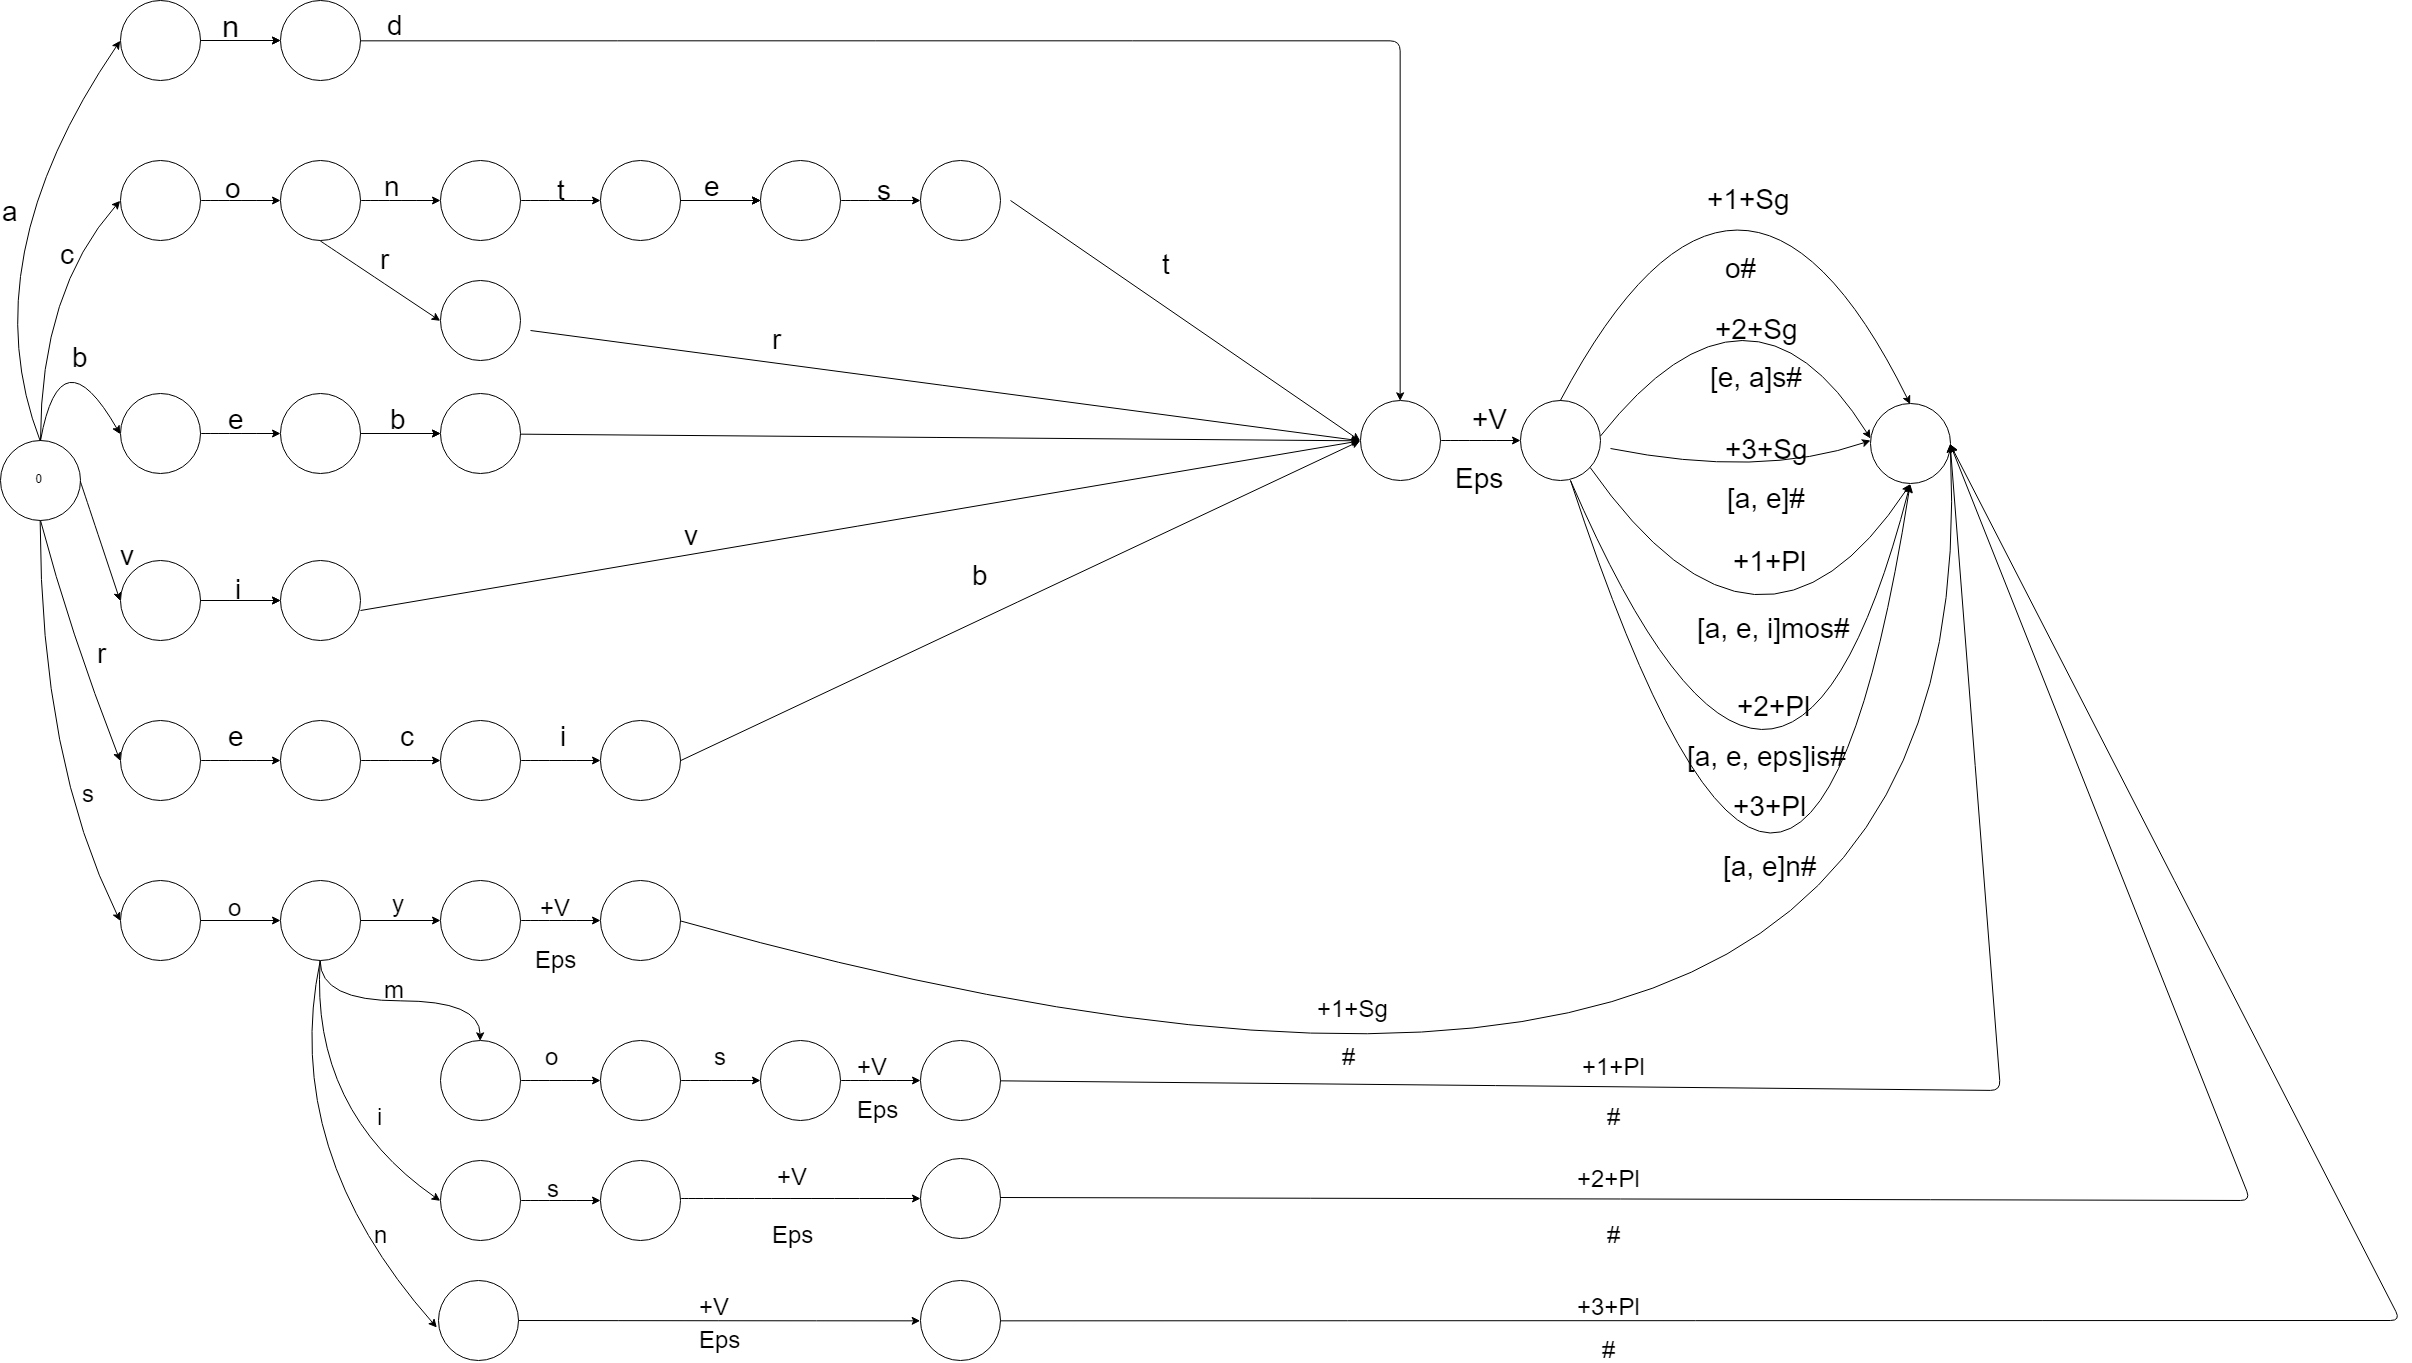
\includegraphics[scale=0.2]{fleshed-out_fst.png}
    \caption{Fleshed-out FST}
    \label{fig:fleshed-out_fst}
\end{figure}

\newpage

\section*{Question 3}

\subsection*{Problem setup}
The goal is to train a binary classifier to perform sentiment analysis on movie reviews. More predisely, the classifier should predict wether a review is positive or negative. The number of examples is equal to 10662. One half of the examples are positive review and the other half of are negative reeviews. The corpus size in 224067 and the lexicon size is 21425. Tree algorithm are compared during the experiment: Naive Bayes, Logistic Regression, and SVM.

\subsection*{Experimental procedure}
The data was split into a training set and a test set. The size of the test set represent 15\% of the data. The test examples are selected randomly among the all the examples. A 5-fold cross-validation procedure was used to select the hyperparameters for each models. During the cross-validation process, a grid search is perform over the predefined set of parameters and the cross-validation is performed on all the different combination of parameters. After the cross-validation process, the hyperparameters that gives the best average accuracy over the 5 folds is selected and refit over all the training set and test on the test set.

\subsection*{Range of parameter setting}

Hyperparameters include parameter for the preprocessing and parameters of the models. All hyperparameters are selected simulaneously since a changing the preprocessing is likely to influence the model behavior. The preprocessor hyperparameters are the number of $n$-grams, the stopwords to remove, the threshold for which unfrequent words are removed (e.g. words that represent less then 0.01\% of the corpus), and the threshold for which too frequent words are removed (e.g. word representing more then 10\% of the copus). The classifier hyperparameters depend on the model. The models hyperparameters that were tuned during cross-validation and there range are shown in tables \ref{table:hyper_preprocess}.

\begin{table}[h!]
    \resizebox{\textwidth}{!}{
    \begin{tabular}{ |cc|cc|cc|cc| } 
        \hline
        Preprocessing & Possible values & SVM & Possible values & Naive Bayes & Possible values & Logistic regression & Possible values \\
        \hline
        $n$-grams & \{1-gram, 2-grams\} & $C$ & \{0.25, 0.5, 0.75, 1, 2, 3, 4, 5\} & $\alpha$ & \{0.5, 0.75, 1., 1.5, 2\} & $C$ & \{0.25, 0.5, 0.75, 1, 2, 3, 4, 5\} \\
        stopwords &  \{none, nltk english stopwords\} & loss function & \{squared hinge\} & & & & \\
        Min frequency threshold & \{none, 0.0001, 0.001\}  & & & & & & \\
        Max frequency threshold & \{none, 0.2, 0.3, 0.4, 0.5\} & & & & & & \\
        \hline
    \end{tabular}}
    \caption{Range of hyperparameters}
    \label{table:hyper_preprocess}
\end{table}


\subsection*{Result and conclusion}
The table \ref{table:result} show the accuracy of the models that performed the best on the training set. The performance are comparable, but the logistic regression perform slightly better. It is surprising that removing a set of stopwords do not improve the accuracy on any models. This indicates that the set of stopwords provided by the library nltk contains more relevant features then unrelevant ones. In particular, nltk list of stopwords include the negative form of some verbs. For instance: haven't, isn't, shouldn't,...These may be useful features to determine wether a review is positive. For example, in "This movie isn't good." the feature "isn't" is very important.

\begin{table}[h!]
    \centering
    \begin{tabular}{ |c|c|c|c| } 
        \hline
        hyperparameters & SVM &		Naive Bayes &		Logistic Regressionm	\\
        \hline
        $n$-grams 	&	2-gram 	&	2-gram	&	2-gram 	\\
        stopwords 	&	None	&	None	&	None	\\
        Min frequency threshold 	&	0.	&	0.	&	0.	\\
        Max frequency threshold 	&	0.4	&	1.	&	0.4	\\
        $C$	&	0.25	&	na & 2.			\\
        $\alpha$	&	na	&	0.75 & na \\			
        train accuracy 	&	0.766	&	0.78	&	0.769	\\
        test accuracy 	&	0.786	&	0.787	&	0.795	\\
        \hline
    \end{tabular}
    \caption{Models accuracy comparison (with there best choice of parameters).}
    \label{table:result}
\end{table} 

\begin{table}[h!]
    \centering
    \begin{tabular}{ |c|c| } 
        \hline
        0.7 & 0.3          
        \hline
        0.2 & 0.8
        \hline
    \end{tabular}
    \caption{Confusion matrix}
    \label{table:result}
\end{table}


\end{document}
